% Created 2022-06-10 Fri 09:49
% Intended LaTeX compiler: pdflatex
\documentclass[11pt]{article}
\usepackage[utf8]{inputenc}
\usepackage[T1]{fontenc}
\usepackage{graphicx}
\usepackage{longtable}
\usepackage{wrapfig}
\usepackage{rotating}
\usepackage[normalem]{ulem}
\usepackage{amsmath}
\usepackage{amssymb}
\usepackage{capt-of}
\usepackage{hyperref}
\usepackage{indentfirst}
\usepackage{amsmath}
\usepackage[margin=3cm]{geometry}
\author{Oscar Morris}
\date{10 Jun 2022}
\title{Block 1}
\hypersetup{
 pdfauthor={Oscar Morris},
 pdftitle={Block 1},
 pdfkeywords={},
 pdfsubject={},
 pdfcreator={Emacs 27.1 (Org mode 9.6)}, 
 pdflang={English}}
\begin{document}

\maketitle


\section{Experiment 1}
\label{sec:org6becf6c}
\subsection{Aims}
\label{sec:org1c85917}
The first set of training was run to establish answers to the following questions:
\begin{enumerate}
\item Can outliers be detected by comparing multiple models?
\begin{itemize}
\item are the outlier answers all the same, or do they change depending on the model?
\end{itemize}
\item How does the distribution of machine-given marks compare with that of the human markers?
\item How do models' predictions compare with each other (similar to question 1)?
\item Do the results found in the EE hold for more repeats and training samples?
\end{enumerate}

\subsection{Planned Method}
\label{sec:orgd6afb42}
Three models were going to be trained on the Tin Iodide synthesis dataset (approx. 100 samples) to determine differences, these models were the highest performing in the EE:
\begin{enumerate}
\item BERT (at the bert-base-cased checkpoint)
\item ALBERT (at the albert-base-v2 checkpoint)
\item Longformer (at the longformer-base-4096 checkpoint)
\end{enumerate}

Each model was trained for 30 epochs with a batch size of 8. Tests were done evaluating the model on unseen data, and on training data.

\subsection{Results}
\label{sec:org93aa199}
During training, the BERT model achieved similar values as in the EE, with \(r^2\) around \(0\) and MAE around 0.1.

\begin{figure}[htbp]
\centering
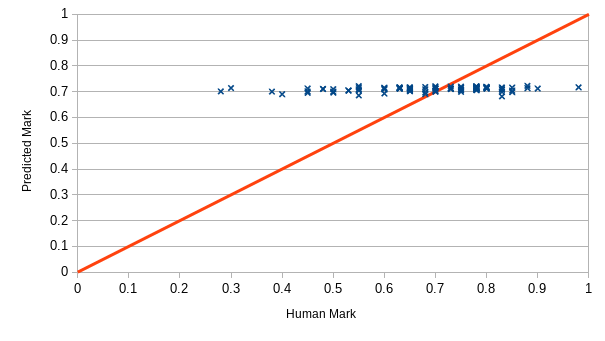
\includegraphics[width=10cm]{./exp1dist.png}
\caption{BERT predictions against Human markers on training data, Orange is the ideal solution \label{fig:bert-dist-mean}}
\end{figure}

As can be seen from Fig. \ref{fig:bert-dist-mean}, the BERT model is always predicting approximately the same value, this value is approximately the mean of the human given marks (\(0.69\)). This is a common issue when training regression models, since most of the time it is better to predict the mean of the training data rather than randomly (and consequently learn the task). On re-examination of the data collected in the EE, it is very likely this this was also occurring in those experiments. This problem is known as ``underfitting,'' either to the training data or to the evaluation data, in this case it appears that the model is underfitting to both splits as the distribution is very similar between seen and unseen samples. Because of this, only the BERT model was trained as the data collected in the EE showed that it was likely this was occurring for all models.

\subsubsection{Cause hypotheses}
\label{sec:orgba02dce}
On the viewing of the data collected in this experiment, a few hypotheses were created for the causes (and potential solutions) to this problem:
\begin{enumerate}
\item The transformer-based models were too large to effectively learn from the data
\item The distribution of human-given marks in the training data was too unbalanced, leading to underfitting.
\item The AES task cannot be effectively learned on this dataset.
\end{enumerate}

\subsubsection{Cause Solutions}
\label{sec:org13af85e}
Possible solutions to each hypothesis are:
\begin{enumerate}
\item Use a smaller pre-trained transformer based on BERT \cite{turcWellReadStudentsLearn2019}, or create and train a small LSTM or self-attention based model
\item Testing on a more balanced dataset, or adjusting the loss metric to account for unbalanced data
\item Testing on a different dataset that has been proven to be effective in previous work.
\end{enumerate}

Each solution has been tested on the Kaggle AES dataset \cite{HewlettFoundationAutomated} in further experiments.

\section{Experiment 2}
\label{sec:org7c5db49}
\subsection{Aims}
\label{sec:org07fe467}
The second experiment aimed to determine the effectiveness of creating, and training a self-attention model from scratch.

\subsection{Methods}
\label{sec:orgf742b00}
The basic model architecture is shown in Fig. \ref{fig:basic-architecture}, with the architecture of the encoder shown in Fig. \ref{fig:encoder-architecture}.

\begin{figure}[htbp]
\centering
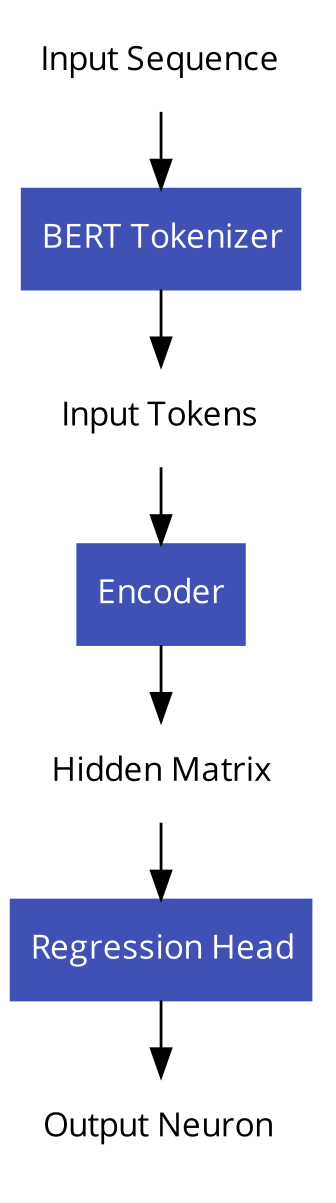
\includegraphics[height=10cm]{../model-basic.png}
\caption{Basic regression transformer architecture \label{fig:basic-architecture}}
\end{figure}

\begin{figure}[htbp]
\centering
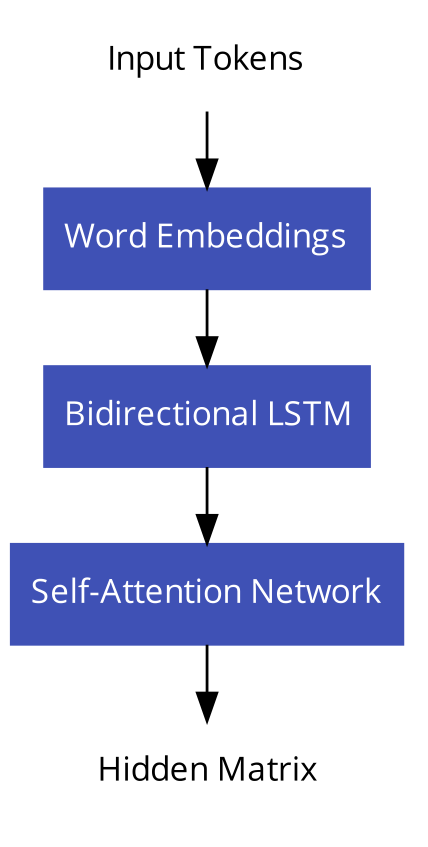
\includegraphics[height=8cm]{../encoder.png}
\caption{Encoder architecture \label{fig:encoder-architecture}}
\end{figure}

Each model was trained for 5 epochs, the model has a hidden LSTM size of 256 and an embedding length of 300.

The model was then pre-trained and evaluated on the Kaggle AES (Automated Essay Scoring) dataset \cite{HewlettFoundationAutomated} and the Kaggle SAS (Short Answer Scoring) dataset \cite{HewlettFoundationShort}.


\newpage

\subsection{Results}
\label{sec:orgd6b9ae6}
The results for this model are very similar to the results for Experiment 1. This shows that the problem likely does not like with the model. However, due to the similar resuts to BERT, this model was used for all further Experiments due to the increase in control and data that a custom model gives.

\section{Experiments 3, 4}
\label{sec:org52acf3e}
No further progress was made in Experiment 3.

In Experiment 4 the model was adjusted slightly, replacing the regression head with a classification head, this was to test the feasibility of a classification system rather than a regression system. Previous work has found it to be ineffective when compared to regression \cite{johanberggrenRegressionClassificationAutomated2019}. However, because of the difficulty in creating a system that allows a regression model to learn effectively it was still attempted. The model achieved a classification accuracy of approximately \(0.6\), almost double what would be expected if the model was guessing randomly, although the model is still not performing well. However, with further tuning and model improvements it is possible that this score could be significantly improved.

\section{Experiment 5}
\label{sec:orgbcf2997}
\subsection{Aims}
\label{sec:orgf6146b6}
Determine the effectiveness of a custom loss metric combining the difference between the standard deviation of the model's predictions and the human marks, and an error metric such as Mean Squared Error (MSE) or Root Mean Squared Error (RMSE). In later versions of the metric \(r^2\) was added.

\subsection{Methods}
\label{sec:org0ecc429}
Metrics are combined to form a single loss function by means of a weighted sum. The importance of a metric in this weighted sum can be defined by some coefficient \(s\):

$$ L_T = s \cdot L_1 + (1-s) \cdot L_2 $$

It was found that the model was unable to optimise both metrics when they were combined with a constant coefficient. Therefore, the coefficient \(s\) was decayed throughout the training process. This significantly improved the performance of the model. The coefficient was then defined using an exponential decay function as follows:

$$ s = e^{-a\frac{t}{T}} $$

where \(a\) is a coefficient determining the rate of decay, \(t\) is the current epoch and \(T\) is the total number of epochs.

This method was found to be much more effective, achieving an \(r^2\) value of approximately 0.1, significantly higher than any previous attempt. This model was only used on the Kaggle AES dataset referenced above.

\begin{figure}[htbp]
\centering
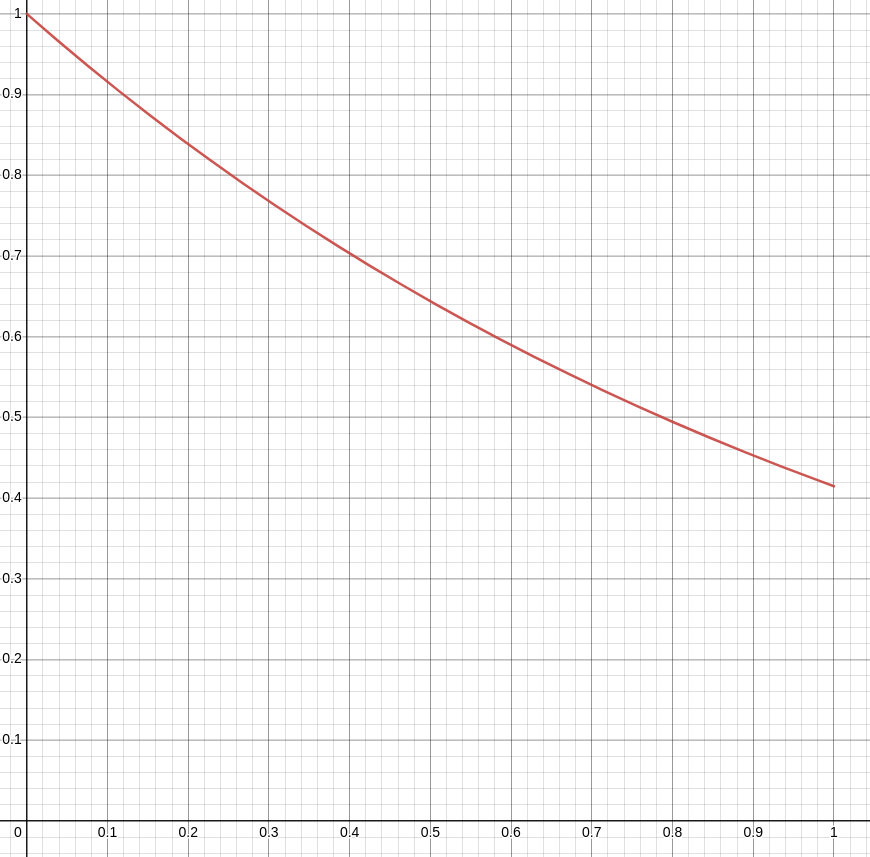
\includegraphics[width=7cm]{./decay_nob.png}
\caption{Graph of \(s\) against \(\frac{t}{T}\), \(a = 0.88\) \label{fig:exponential_nob}}
\end{figure}

During the training of this model, the difference between the predicted and human standard deviations remained relatively high, much higher than expected. Therefore, it was decided to redefine the decay curve to allow the model more time to focus on the achieving the correct standard devaiation. Therefore, \(s\) was defined as a piecewise function as follows:

\[ s = \begin{cases}
c & 0\leq \frac{t}{T} \leq b \\
c \cdot e^{-a(\frac{t}{T} - b)} & b \leq \frac{t}{T} \leq 1
\end{cases} \]

where \(c\) is the starting value of \(s\) (usually set to \(1\)) and \(b\) is the point at which the function begins to decay

\begin{figure}[htbp]
\centering
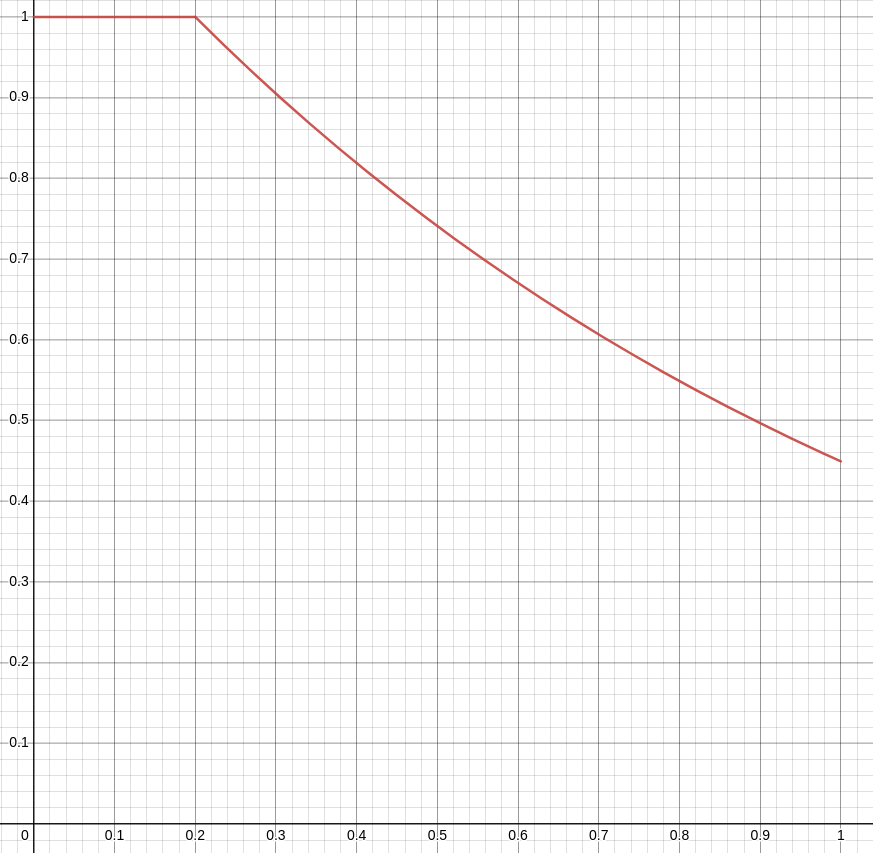
\includegraphics[width=7cm]{./decay_wb.png}
\caption{Graph of \(s\) against \(\frac{t}{T}\), \(a=1\), \(b=0.2\), \(c=1\) \label{fig:exponential_wb}}
\end{figure}

The individual loss functions (after \(r^2\) was added) are defined as follows:

$$ L_1 = \abs(\sigma_{pred} - \sigma_{true}) $$

$$ L_2 = \text{RMSE}-d \cdot r^2 $$

where \(\sigma_{pred}\) is the standard deviation of the predicted values, \(\sigma_{true}\) is the standard deviation of the human given values, \(d\) is a constant coefficient and \(r^2\) is the coefficient of determination.

The best performing models were trained for \(200\) epochs using a batch size of \(64\), however, no hyperparameter tuning has been executed. The model used has a hidden LSTM size of 512 and an embedding length of 128 giving approximately 70 million trainable parameters.

\subsection{Results}
\label{sec:orgce74f69}
The model final model evaluated in this experiment beats all other attempts achieving an \(r^2\) score approaching (and occasionally exceeding) \(0.6\) on both Kaggle datasets.

\begin{figure}[htbp]
\centering
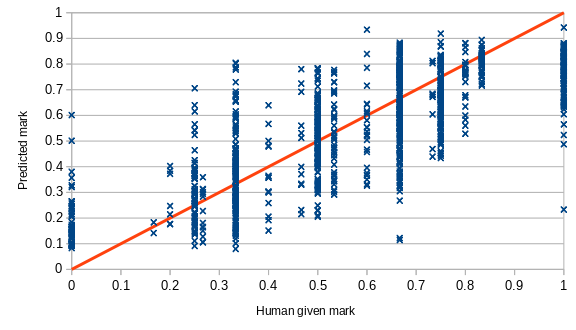
\includegraphics[width=10cm]{./exp5_aes_dist.png}
\caption{Predicted score against Human given score on a run achieving \(r^2 \approx 0.58\)}
\end{figure}

The model trained on the AES dataset was then further trained on the SAS dataset. It was found that the model pre-trained on the AES dataset performed worse than when the model was trained completely on the SAS dataset. However, when the model was pre-trained it could consistently achieve performance slightly lower than the better performing pure SAS models, average performance for both model has not yet been calculated.

The model trained only on the SAS dataset performed very well achieving an \(r^2\) of approximately 0.63.

\begin{figure}[htbp]
\centering
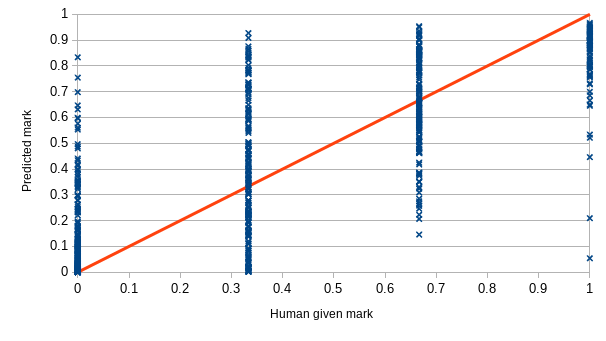
\includegraphics[width=10cm]{./exp5_sas_dist.png}
\caption{Predicted score against Human given score on a run trained on SAS}
\end{figure}

\begin{figure}[htbp]
\centering
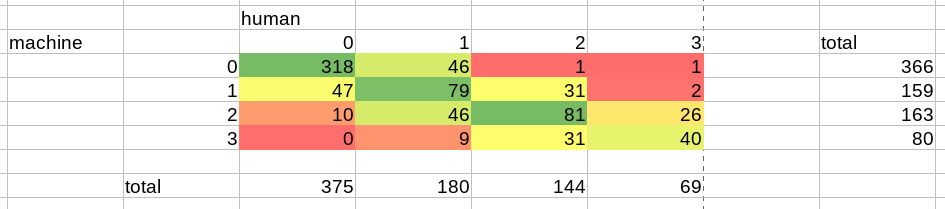
\includegraphics[width=10cm]{./exp5_sas_confusion.png}
\caption{Confusion matrix for SAS data}
\end{figure}

During the training it was found that this metric performs significantly better when training using a high batch size. This is likely because it makes the standard deviation and coefficient of determination more analogous to what the model would predict in a real world setting and can, therefore, better optimise the model for this task.

\newpage

\section{Conclusion}
\label{sec:org89a18dc}
The models created in this block (length: 2 weeks) have shown significant improvement over previous attempts using transformer models for AES and show significant promise using the Kaggle datasets as a pre-training method to create a pre-training framework specific to AES, allowing for fewer samples to be used when fine-tuning a model for a real-world application.

The pre-training step is time-efficient as the model is able to achieve comparatively high performance in just over an hour of training (on \textbf{\textbf{either}} the Kaggle AES dataset \textbf{\textbf{or}} the Kaggle SAS dataset).

These results show great promise when it is considered that the hyperparameters presented here have not been tuned but only roughly estimated. Therefore, it is reasonable to suggest that with hyperparameter tuning the models could perform significantly better than presented here.

\bibliographystyle{ieeetr}
\bibliography{../bibliography}
\end{document}
